% Graphic for TeX using PGF
% Title: /home/lluis/Escritorio/TFM/Informe/images/model_object_diagram.dia
% Creator: Dia v0.97.2
% CreationDate: Thu May 19 11:39:34 2016
% For: lluis
% \usepackage{tikz}
% The following commands are not supported in PSTricks at present
% We define them conditionally, so when they are implemented,
% this pgf file will use them.
\ifx\du\undefined
  \newlength{\du}
\fi
\setlength{\du}{15\unitlength}
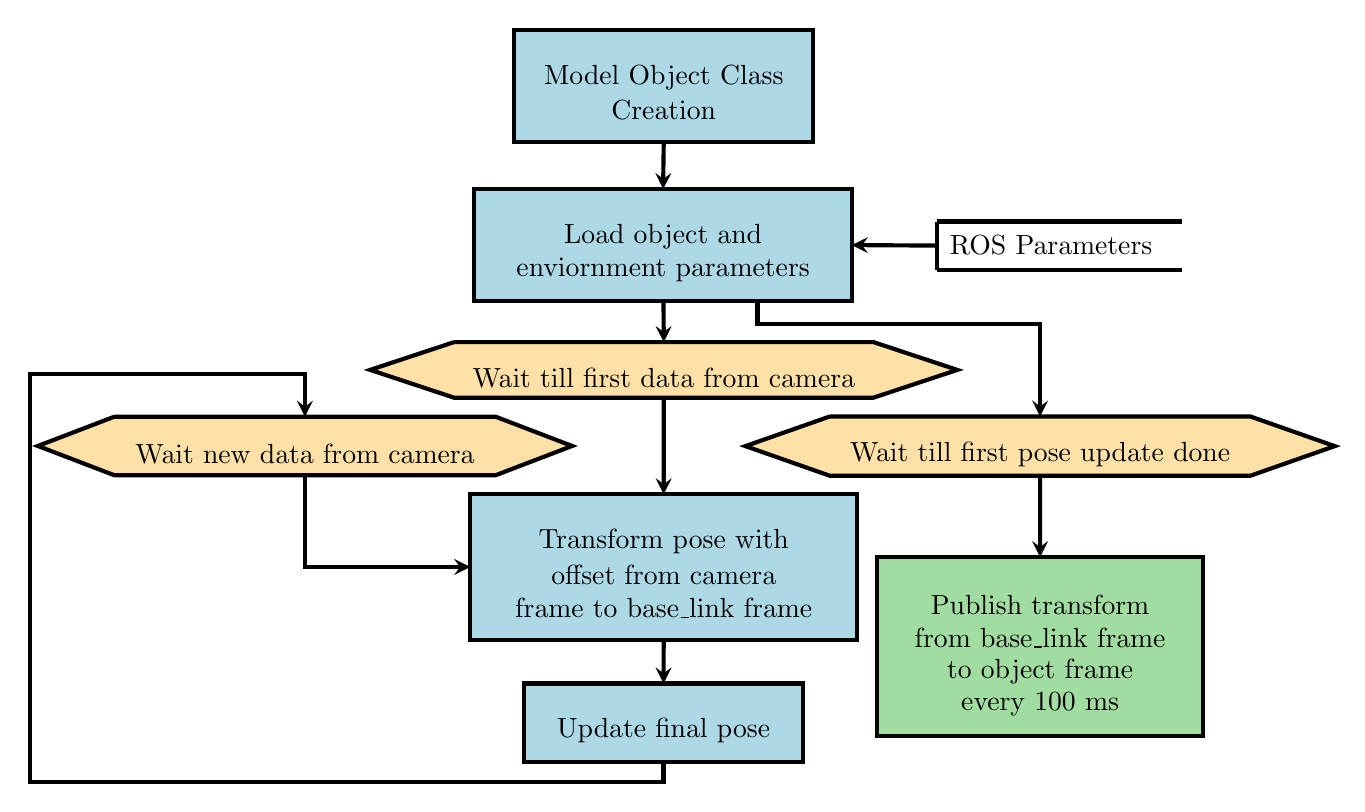
\begin{tikzpicture}
\pgftransformxscale{1.000000}
\pgftransformyscale{-1.000000}
\definecolor{dialinecolor}{rgb}{0.000000, 0.000000, 0.000000}
\pgfsetstrokecolor{dialinecolor}
\definecolor{dialinecolor}{rgb}{1.000000, 1.000000, 1.000000}
\pgfsetfillcolor{dialinecolor}
\definecolor{dialinecolor}{rgb}{0.678431, 0.847059, 0.901961}
\pgfsetfillcolor{dialinecolor}
\fill (12.205200\du,4.120720\du)--(12.205200\du,6.820720\du)--(19.405200\du,6.820720\du)--(19.405200\du,4.120720\du)--cycle;
\pgfsetlinewidth{0.100000\du}
\pgfsetdash{}{0pt}
\pgfsetdash{}{0pt}
\pgfsetmiterjoin
\definecolor{dialinecolor}{rgb}{0.000000, 0.000000, 0.000000}
\pgfsetstrokecolor{dialinecolor}
\draw (12.205200\du,4.120720\du)--(12.205200\du,6.820720\du)--(19.405200\du,6.820720\du)--(19.405200\du,4.120720\du)--cycle;
% setfont left to latex
\definecolor{dialinecolor}{rgb}{0.000000, 0.000000, 0.000000}
\pgfsetstrokecolor{dialinecolor}
\node at (15.805200\du,5.265720\du){Model Object Class};
% setfont left to latex
\definecolor{dialinecolor}{rgb}{0.000000, 0.000000, 0.000000}
\pgfsetstrokecolor{dialinecolor}
\node at (15.805200\du,6.065720\du){Creation};
\definecolor{dialinecolor}{rgb}{0.678431, 0.847059, 0.901961}
\pgfsetfillcolor{dialinecolor}
\fill (11.242800\du,7.957890\du)--(11.242800\du,10.657890\du)--(20.337800\du,10.657890\du)--(20.337800\du,7.957890\du)--cycle;
\pgfsetlinewidth{0.100000\du}
\pgfsetdash{}{0pt}
\pgfsetdash{}{0pt}
\pgfsetmiterjoin
\definecolor{dialinecolor}{rgb}{0.000000, 0.000000, 0.000000}
\pgfsetstrokecolor{dialinecolor}
\draw (11.242800\du,7.957890\du)--(11.242800\du,10.657890\du)--(20.337800\du,10.657890\du)--(20.337800\du,7.957890\du)--cycle;
% setfont left to latex
\definecolor{dialinecolor}{rgb}{0.000000, 0.000000, 0.000000}
\pgfsetstrokecolor{dialinecolor}
\node at (15.790300\du,9.102890\du){Load object and};
% setfont left to latex
\definecolor{dialinecolor}{rgb}{0.000000, 0.000000, 0.000000}
\pgfsetstrokecolor{dialinecolor}
\node at (15.790300\du,9.902890\du){enviornment parameters};
\pgfsetlinewidth{0.100000\du}
\pgfsetdash{}{0pt}
\pgfsetdash{}{0pt}
\pgfsetbuttcap
\pgfsetmiterjoin
\pgfsetlinewidth{0.100000\du}
\pgfsetbuttcap
\pgfsetmiterjoin
\pgfsetdash{}{0pt}
\definecolor{dialinecolor}{rgb}{1.000000, 0.878431, 0.650980}
\pgfsetfillcolor{dialinecolor}
\pgfpathmoveto{\pgfpoint{10.754810\du}{11.645500\du}}
\pgfpathlineto{\pgfpoint{20.857310\du}{11.645500\du}}
\pgfpathlineto{\pgfpoint{22.877810\du}{12.314734\du}}
\pgfpathlineto{\pgfpoint{20.857310\du}{12.983968\du}}
\pgfpathlineto{\pgfpoint{10.754810\du}{12.983968\du}}
\pgfpathlineto{\pgfpoint{8.734310\du}{12.314734\du}}
\pgfpathlineto{\pgfpoint{10.754810\du}{11.645500\du}}
\pgfusepath{fill}
\definecolor{dialinecolor}{rgb}{0.000000, 0.000000, 0.000000}
\pgfsetstrokecolor{dialinecolor}
\pgfpathmoveto{\pgfpoint{10.754810\du}{11.645500\du}}
\pgfpathlineto{\pgfpoint{20.857310\du}{11.645500\du}}
\pgfpathlineto{\pgfpoint{22.877810\du}{12.314734\du}}
\pgfpathlineto{\pgfpoint{20.857310\du}{12.983968\du}}
\pgfpathlineto{\pgfpoint{10.754810\du}{12.983968\du}}
\pgfpathlineto{\pgfpoint{8.734310\du}{12.314734\du}}
\pgfpathlineto{\pgfpoint{10.754810\du}{11.645500\du}}
\pgfusepath{stroke}
% setfont left to latex
\definecolor{dialinecolor}{rgb}{0.000000, 0.000000, 0.000000}
\pgfsetstrokecolor{dialinecolor}
\node at (15.806060\du,12.514734\du){Wait till first data from camera};
\definecolor{dialinecolor}{rgb}{0.678431, 0.847059, 0.901961}
\pgfsetfillcolor{dialinecolor}
\fill (11.142100\du,15.311400\du)--(11.142100\du,18.811400\du)--(20.467100\du,18.811400\du)--(20.467100\du,15.311400\du)--cycle;
\pgfsetlinewidth{0.100000\du}
\pgfsetdash{}{0pt}
\pgfsetdash{}{0pt}
\pgfsetmiterjoin
\definecolor{dialinecolor}{rgb}{0.000000, 0.000000, 0.000000}
\pgfsetstrokecolor{dialinecolor}
\draw (11.142100\du,15.311400\du)--(11.142100\du,18.811400\du)--(20.467100\du,18.811400\du)--(20.467100\du,15.311400\du)--cycle;
% setfont left to latex
\definecolor{dialinecolor}{rgb}{0.000000, 0.000000, 0.000000}
\pgfsetstrokecolor{dialinecolor}
\node at (15.804600\du,16.456400\du){Transform pose with};
% setfont left to latex
\definecolor{dialinecolor}{rgb}{0.000000, 0.000000, 0.000000}
\pgfsetstrokecolor{dialinecolor}
\node at (15.804600\du,17.256400\du){offset from camera};
% setfont left to latex
\definecolor{dialinecolor}{rgb}{0.000000, 0.000000, 0.000000}
\pgfsetstrokecolor{dialinecolor}
\node at (15.804600\du,18.056400\du){ frame to base\_link frame};
\pgfsetlinewidth{0.100000\du}
\pgfsetdash{}{0pt}
\pgfsetdash{}{0pt}
\pgfsetmiterjoin
\pgfsetbuttcap
{
\definecolor{dialinecolor}{rgb}{0.000000, 0.000000, 0.000000}
\pgfsetfillcolor{dialinecolor}
% was here!!!
\pgfsetarrowsend{stealth}
{\pgfsetcornersarced{\pgfpoint{0.000000\du}{0.000000\du}}\definecolor{dialinecolor}{rgb}{0.000000, 0.000000, 0.000000}
\pgfsetstrokecolor{dialinecolor}
\draw (18.064100\du,10.657900\du)--(18.064100\du,11.218100\du)--(24.871345\du,11.218100\du)--(24.871345\du,13.438275\du);
}}
\definecolor{dialinecolor}{rgb}{0.678431, 0.847059, 0.901961}
\pgfsetfillcolor{dialinecolor}
\fill (12.434900\du,19.868500\du)--(12.434900\du,21.768500\du)--(19.164900\du,21.768500\du)--(19.164900\du,19.868500\du)--cycle;
\pgfsetlinewidth{0.100000\du}
\pgfsetdash{}{0pt}
\pgfsetdash{}{0pt}
\pgfsetmiterjoin
\definecolor{dialinecolor}{rgb}{0.000000, 0.000000, 0.000000}
\pgfsetstrokecolor{dialinecolor}
\draw (12.434900\du,19.868500\du)--(12.434900\du,21.768500\du)--(19.164900\du,21.768500\du)--(19.164900\du,19.868500\du)--cycle;
% setfont left to latex
\definecolor{dialinecolor}{rgb}{0.000000, 0.000000, 0.000000}
\pgfsetstrokecolor{dialinecolor}
\node at (15.799900\du,21.013500\du){Update final pose};
\definecolor{dialinecolor}{rgb}{0.631373, 0.862745, 0.631373}
\pgfsetfillcolor{dialinecolor}
\fill (20.938445\du,16.826200\du)--(20.938445\du,21.126200\du)--(28.805945\du,21.126200\du)--(28.805945\du,16.826200\du)--cycle;
\pgfsetlinewidth{0.100000\du}
\pgfsetdash{}{0pt}
\pgfsetdash{}{0pt}
\pgfsetmiterjoin
\definecolor{dialinecolor}{rgb}{0.000000, 0.000000, 0.000000}
\pgfsetstrokecolor{dialinecolor}
\draw (20.938445\du,16.826200\du)--(20.938445\du,21.126200\du)--(28.805945\du,21.126200\du)--(28.805945\du,16.826200\du)--cycle;
% setfont left to latex
\definecolor{dialinecolor}{rgb}{0.000000, 0.000000, 0.000000}
\pgfsetstrokecolor{dialinecolor}
\node at (24.872195\du,17.971200\du){Publish transform };
% setfont left to latex
\definecolor{dialinecolor}{rgb}{0.000000, 0.000000, 0.000000}
\pgfsetstrokecolor{dialinecolor}
\node at (24.872195\du,18.771200\du){from base\_link frame};
% setfont left to latex
\definecolor{dialinecolor}{rgb}{0.000000, 0.000000, 0.000000}
\pgfsetstrokecolor{dialinecolor}
\node at (24.872195\du,19.571200\du){to object frame};
% setfont left to latex
\definecolor{dialinecolor}{rgb}{0.000000, 0.000000, 0.000000}
\pgfsetstrokecolor{dialinecolor}
\node at (24.872195\du,20.371200\du){every 100 ms};
\pgfsetlinewidth{0.100000\du}
\pgfsetdash{}{0pt}
\pgfsetdash{}{0pt}
\pgfsetbuttcap
{
\definecolor{dialinecolor}{rgb}{0.000000, 0.000000, 0.000000}
\pgfsetfillcolor{dialinecolor}
% was here!!!
\pgfsetarrowsend{stealth}
\definecolor{dialinecolor}{rgb}{0.000000, 0.000000, 0.000000}
\pgfsetstrokecolor{dialinecolor}
\draw (15.804600\du,18.811400\du)--(15.799900\du,19.868500\du);
}
\pgfsetlinewidth{0.100000\du}
\pgfsetdash{}{0pt}
\pgfsetdash{}{0pt}
\pgfsetbuttcap
{
\definecolor{dialinecolor}{rgb}{0.000000, 0.000000, 0.000000}
\pgfsetfillcolor{dialinecolor}
% was here!!!
\pgfsetarrowsend{stealth}
\definecolor{dialinecolor}{rgb}{0.000000, 0.000000, 0.000000}
\pgfsetstrokecolor{dialinecolor}
\draw (24.871345\du,14.863417\du)--(24.872195\du,16.826200\du);
}
\pgfsetlinewidth{0.100000\du}
\pgfsetdash{}{0pt}
\pgfsetdash{}{0pt}
\pgfsetbuttcap
\pgfsetmiterjoin
\pgfsetlinewidth{0.100000\du}
\pgfsetbuttcap
\pgfsetmiterjoin
\pgfsetdash{}{0pt}
\definecolor{dialinecolor}{rgb}{1.000000, 0.878431, 0.650980}
\pgfsetfillcolor{dialinecolor}
\pgfpathmoveto{\pgfpoint{19.801345\du}{13.438275\du}}
\pgfpathlineto{\pgfpoint{29.941345\du}{13.438275\du}}
\pgfpathlineto{\pgfpoint{31.969345\du}{14.150846\du}}
\pgfpathlineto{\pgfpoint{29.941345\du}{14.863417\du}}
\pgfpathlineto{\pgfpoint{19.801345\du}{14.863417\du}}
\pgfpathlineto{\pgfpoint{17.773345\du}{14.150846\du}}
\pgfpathlineto{\pgfpoint{19.801345\du}{13.438275\du}}
\pgfusepath{fill}
\definecolor{dialinecolor}{rgb}{0.000000, 0.000000, 0.000000}
\pgfsetstrokecolor{dialinecolor}
\pgfpathmoveto{\pgfpoint{19.801345\du}{13.438275\du}}
\pgfpathlineto{\pgfpoint{29.941345\du}{13.438275\du}}
\pgfpathlineto{\pgfpoint{31.969345\du}{14.150846\du}}
\pgfpathlineto{\pgfpoint{29.941345\du}{14.863417\du}}
\pgfpathlineto{\pgfpoint{19.801345\du}{14.863417\du}}
\pgfpathlineto{\pgfpoint{17.773345\du}{14.150846\du}}
\pgfpathlineto{\pgfpoint{19.801345\du}{13.438275\du}}
\pgfusepath{stroke}
% setfont left to latex
\definecolor{dialinecolor}{rgb}{0.000000, 0.000000, 0.000000}
\pgfsetstrokecolor{dialinecolor}
\node at (24.871345\du,14.350846\du){Wait till first pose update done};
\pgfsetlinewidth{0.100000\du}
\pgfsetdash{}{0pt}
\pgfsetdash{}{0pt}
\pgfsetbuttcap
\pgfsetmiterjoin
\pgfsetlinewidth{0.100000\du}
\pgfsetbuttcap
\pgfsetmiterjoin
\pgfsetdash{}{0pt}
\definecolor{dialinecolor}{rgb}{1.000000, 0.878431, 0.650980}
\pgfsetfillcolor{dialinecolor}
\pgfpathmoveto{\pgfpoint{2.566605\du}{13.443649\du}}
\pgfpathlineto{\pgfpoint{11.759105\du}{13.443649\du}}
\pgfpathlineto{\pgfpoint{13.597605\du}{14.147320\du}}
\pgfpathlineto{\pgfpoint{11.759105\du}{14.850991\du}}
\pgfpathlineto{\pgfpoint{2.566605\du}{14.850991\du}}
\pgfpathlineto{\pgfpoint{0.728105\du}{14.147320\du}}
\pgfpathlineto{\pgfpoint{2.566605\du}{13.443649\du}}
\pgfusepath{fill}
\definecolor{dialinecolor}{rgb}{0.000000, 0.000000, 0.000000}
\pgfsetstrokecolor{dialinecolor}
\pgfpathmoveto{\pgfpoint{2.566605\du}{13.443649\du}}
\pgfpathlineto{\pgfpoint{11.759105\du}{13.443649\du}}
\pgfpathlineto{\pgfpoint{13.597605\du}{14.147320\du}}
\pgfpathlineto{\pgfpoint{11.759105\du}{14.850991\du}}
\pgfpathlineto{\pgfpoint{2.566605\du}{14.850991\du}}
\pgfpathlineto{\pgfpoint{0.728105\du}{14.147320\du}}
\pgfpathlineto{\pgfpoint{2.566605\du}{13.443649\du}}
\pgfusepath{stroke}
% setfont left to latex
\definecolor{dialinecolor}{rgb}{0.000000, 0.000000, 0.000000}
\pgfsetstrokecolor{dialinecolor}
\node at (7.162855\du,14.347320\du){Wait new data from camera};
\pgfsetlinewidth{0.100000\du}
\pgfsetdash{}{0pt}
\pgfsetdash{}{0pt}
\pgfsetmiterjoin
\pgfsetbuttcap
{
\definecolor{dialinecolor}{rgb}{0.000000, 0.000000, 0.000000}
\pgfsetfillcolor{dialinecolor}
% was here!!!
\pgfsetarrowsend{stealth}
{\pgfsetcornersarced{\pgfpoint{0.000000\du}{0.000000\du}}\definecolor{dialinecolor}{rgb}{0.000000, 0.000000, 0.000000}
\pgfsetstrokecolor{dialinecolor}
\draw (15.799900\du,21.768500\du)--(15.799900\du,22.233800\du)--(0.532559\du,22.233800\du)--(0.532559\du,12.405408\du)--(7.162855\du,12.405408\du)--(7.162855\du,13.443649\du);
}}
\pgfsetlinewidth{0.100000\du}
\pgfsetdash{}{0pt}
\pgfsetdash{}{0pt}
\pgfsetmiterjoin
\pgfsetbuttcap
{
\definecolor{dialinecolor}{rgb}{0.000000, 0.000000, 0.000000}
\pgfsetfillcolor{dialinecolor}
% was here!!!
\pgfsetarrowsend{stealth}
{\pgfsetcornersarced{\pgfpoint{0.000000\du}{0.000000\du}}\definecolor{dialinecolor}{rgb}{0.000000, 0.000000, 0.000000}
\pgfsetstrokecolor{dialinecolor}
\draw (7.162855\du,14.850991\du)--(7.162855\du,17.061400\du)--(11.142100\du,17.061400\du);
}}
\pgfsetlinewidth{0.100000\du}
\pgfsetdash{}{0pt}
\pgfsetdash{}{0pt}
\pgfsetbuttcap
{
\definecolor{dialinecolor}{rgb}{0.000000, 0.000000, 0.000000}
\pgfsetfillcolor{dialinecolor}
% was here!!!
\pgfsetarrowsend{stealth}
\definecolor{dialinecolor}{rgb}{0.000000, 0.000000, 0.000000}
\pgfsetstrokecolor{dialinecolor}
\draw (15.806100\du,12.983900\du)--(15.804600\du,15.311400\du);
}
\pgfsetlinewidth{0.100000\du}
\pgfsetdash{}{0pt}
\pgfsetdash{}{0pt}
\pgfsetbuttcap
{
\definecolor{dialinecolor}{rgb}{0.000000, 0.000000, 0.000000}
\pgfsetfillcolor{dialinecolor}
% was here!!!
\pgfsetarrowsend{stealth}
\definecolor{dialinecolor}{rgb}{0.000000, 0.000000, 0.000000}
\pgfsetstrokecolor{dialinecolor}
\draw (15.799762\du,10.707831\du)--(15.806100\du,11.645500\du);
}
\pgfsetlinewidth{0.100000\du}
\pgfsetdash{}{0pt}
\pgfsetdash{}{0pt}
\pgfsetbuttcap
{
\definecolor{dialinecolor}{rgb}{0.000000, 0.000000, 0.000000}
\pgfsetfillcolor{dialinecolor}
% was here!!!
\pgfsetarrowsend{stealth}
\definecolor{dialinecolor}{rgb}{0.000000, 0.000000, 0.000000}
\pgfsetstrokecolor{dialinecolor}
\draw (15.805200\du,6.820720\du)--(15.790300\du,7.957890\du);
}
\pgfsetlinewidth{0.100000\du}
\pgfsetdash{}{0pt}
\pgfsetdash{}{0pt}
\pgfsetbuttcap
\pgfsetmiterjoin
\pgfsetlinewidth{0.100000\du}
\pgfsetbuttcap
\pgfsetmiterjoin
\pgfsetdash{}{0pt}
\definecolor{dialinecolor}{rgb}{0.000000, 0.000000, 0.000000}
\pgfsetstrokecolor{dialinecolor}
\draw (22.396300\du,8.741380\du)--(22.396300\du,9.899275\du);
\pgfsetbuttcap
\pgfsetmiterjoin
\pgfsetdash{}{0pt}
\definecolor{dialinecolor}{rgb}{0.000000, 0.000000, 0.000000}
\pgfsetstrokecolor{dialinecolor}
\draw (22.396300\du,8.741380\du)--(28.284830\du,8.741380\du);
\pgfsetbuttcap
\pgfsetmiterjoin
\pgfsetdash{}{0pt}
\definecolor{dialinecolor}{rgb}{0.000000, 0.000000, 0.000000}
\pgfsetstrokecolor{dialinecolor}
\draw (22.396300\du,9.899275\du)--(28.284830\du,9.899275\du);
% setfont left to latex
\definecolor{dialinecolor}{rgb}{0.000000, 0.000000, 0.000000}
\pgfsetstrokecolor{dialinecolor}
\node at (25.487778\du,9.549275\du){};
% setfont left to latex
\definecolor{dialinecolor}{rgb}{0.000000, 0.000000, 0.000000}
\pgfsetstrokecolor{dialinecolor}
\node[anchor=west] at (22.423900\du,9.302650\du){ROS Parameters};
\pgfsetlinewidth{0.100000\du}
\pgfsetdash{}{0pt}
\pgfsetdash{}{0pt}
\pgfsetbuttcap
{
\definecolor{dialinecolor}{rgb}{0.000000, 0.000000, 0.000000}
\pgfsetfillcolor{dialinecolor}
% was here!!!
\pgfsetarrowsend{stealth}
\definecolor{dialinecolor}{rgb}{0.000000, 0.000000, 0.000000}
\pgfsetstrokecolor{dialinecolor}
\draw (22.396300\du,9.320320\du)--(20.337800\du,9.307890\du);
}
\end{tikzpicture}
